\chapter{Lyapunov-based approach}

JuPE performs algorithm analysis by using the technique layed out by Van Scoy and Lessard in \cite{tutorial}. While JuPE is a blackbox tool, understanding the mathematical approach on which it is based is prequisite to understanding the package's code and functionalities.

The steps of this technique, which will be discussed in detail over the sections of this chapter, consists of 1) viewing the algorithm as a Lur'e problem, 2) Replacing the nonlinear gradient with interpolation conditions that represent the class of smooth strongly convex functions, 3) Use lifting matrices to tighten to the interpolation condition representations, and 4) Prove whether a convergence rate is guaranteed by solving a convex semidefinte program.
%%%%%%%%%%%%%%%%%%%%%%%%%%%%%%%%%%%%%%%%%%%%%%%%%%%%%%%%%%%%%%%%%%%%%%%%%%%%%%%%
\section{Iterative algorithms as Lur'e problems}

The first step in the technique is to view optimization algorithms from a control theory perspective: As iterative gradient-based algorithms uses the gradient of the function to update \(x\), they can be reformulated into a linear time-invariant (LTI) system (how the algorithm update) in feedback with a static nonlinearity (the gradient of \(f\)) at point \(x\). Using a block diagram, the algorithm can be seen as:

\begin{figure}[h]
    \centering
	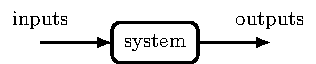
\includegraphics[width = .3 \textwidth]{block-diagram}
    \caption{Block diagram representation of iterative algorithms}
    \label{plot_result}
\end{figure}

Here, \(G\) represents the LTI system, while \(y\) and \(u\) are input and output of the gradient nonlinearity. For example, (FG) equation \ref{eqn:FG} can be rewritten to match this view as:
\begin{subequations} \label{eqn:FG2}
	\begin{align}
	  x_{k+1}     &=x_k-\alpha u_k \label{eq_FGstate},       \\
	  y_{k+1} &=x_{k+1}+\beta (x_{k+1}-x_k), \label{eq_FGinterpolated point}, \\
	  u_k &= \nabla f(y_k) \label{eq_FGggradient}
	\end{align}
	\end{subequations}
The algorithm can then be put into state-space representation as:
\begin{subequations} \label{eqn:FGss }
	\begin{align}
	  \xi_{k+1} &= \bmat{(1+\beta) & -\beta\\ 1 & 0}\xi_k  + \bmat{-\alpha\\ 0}u_k \label{eq_FGssstate}, \\
	  y_k &= \bmat{1+\beta & \beta}\xi_k, \label{eq_FGssinterpolation},\\
	  u_k &= \nabla f(y_k) \label{eq_FGssgradient}
	\end{align}
	\end{subequations}

The LTI system \(G\) can be expressed with four matrices that change in value depending on the algorithm and size depending on the number of past states used to update \(x\). For (GD), (FG), and (HB) as they are described in 1.1, these matrices are:

Beyond the three listed examples, this step can be applied to any other first order methods. Deriving an LTI system represented by matrices out of an algorithm not only creates a representation easy to understand and operate on, but also in next sections enable the representation of the past states of an algorithm and the forming of a Lyapunov function that will guarantee a convergence rate.

\section{Interpolation condition}

For the remainder of this paper, we will focus on the only class of function currently supported by JuPE, m strong L smooth convex function \(f \in \) \(F_{m,L}\).

In the field of robust control theory utilized by this Lyapunov-based approach, while an LTI system is relatively simple, the nonlinearity representing the gradient of the function cannot be efficiently solved. As a result, our approach replaces the nonlinearity with a set of conditions on its input and output, which provides necessary and sufficient conditions under which there exists a function \(f \in \) \(F_{m,L}\) that interpolates a given finite set of argument-function value-gradient triplets. These interpolation conditions depends on the characteristics of the function class and was first formulated in \cite{taylor2016} and reformatted in \cite{tutorial}:

\begin{theorem}[\cite{taylor2016}, Thm. 4; \cite{tutorial}, Thm. 3]
	\label{thm:interpolation_condition}
	Given index set \(I\), a set of triplets \({(y_k, u_k, f_k)}_{k \in I}\) is \(F_{m,L}-interpolable\), meaning there exists a function \(f \in F_{m,L}\) satisfying \(f(y_k) = f_k\) and \(\nabla f(y_k) = u_k\) if and only if:

	\(2(L-m)(f_i - f_j) - mL||y_i - y_j||^2 + 2(y_i - y_j)^{T}(mu_i - Lu_j) - ||u_i - u_j||^2 > 0\) for \(i ,j \in I\)

\end{theorem}

Where the Euclidean-norm of a vector \(x\) is denoted as \(||x||\). Basing on this theorem, [\cite{tutorial}, Cor 4] presented a non-negative linear combination of inequalities to create a tight representation of the class of function, which can be rewritten in a way easier to implement into code as:

\begin{corollary}[\cite{tutorial}, Cor. 4]
	Given a function \(f \in F_{m,L}\) and let \(y_k,...,y_{k-l}\) be a sequence of iterates; \(u_{k-i} = \nabla f(y_{k-i})\) and \(f_{k-i} = f(y_{k-i})\) for \(i \in 0,...l\). Then the inequality:
	
	holds for all \(\Lambda \in \mathbb{R}^{(l+2) * (l+2)}\) and \(\Lambda >= 0\), and \(\Pi(\Lambda)\) and  \(\pi(\Lambda)\) are defined as:

\end{corollary}

This step in the methodology is similar to that in \cite{pepit}. By using interpolation conditions, the gradient of smooth strongly convex class of function inputted is represented by non-negative inequalities. This combined with the use of Lyapunov-functions to prove convergence rate which will be presented in 3.4 allows analysis to be done be solving a convex program

\section{Lifting algorithm}

\section{Lyapunov function certification}
\begin{equation} \label{eqn:Lyapunov}
	V(x) = <P, X[x; u]> = <X^T P, [x; u]>
\end{equation}

